\chapter{الصبغين وعلم اللاجينات}\label{ch:b3:chromatin-epigenetics}

فأران من بطن واحدة، متطابقان وراثيًا حتى آخر قاعدة، يجلسان جنبًا إلى
جنب: أحدهما نحيل بني، والآخر بدين أصفر سيصاب بالسكري. وقطة كاليكو
تلبس بقعًا برتقالية وسوداء مع أن كل خلية من جلدها تحمل الصبغيين
الجنسيين X نفسيهما. وطفل يرث من الصبغي 15 القطعة المحذوفة نفسها التي
ورثها طفل آخر، فيصاب أحدهما بمتلازمة برادر--فيلي ويصاب الآخر بمتلازمة
أنجلمان --- والفارق الوحيد هو من أي الأبوين جاء الحذف. لا شيء من هذا
مكتوب في تسلسل DNA، بل هو مكتوب \emph{عليه}: في الطريقة التي يُرصّ
بها مترا DNA في نواة قطرها عشرة ميكرومترات، وفي الزمر الكيميائية
الصغيرة الملتصقة ببروتينات الرص وبالسيتوزينات نفسها، وفي الآلية التي
تنسخ تلك العلامات من خلية إلى بناتها. يتناول هذا الفصل تلك الطبقة
الثانية من المعلومات، وحواملها الجزيئية، والحدود الصادقة لما تستطيع
أن تتذكره.

\section{الصبغين: DNA على بكرة}

\begin{definition}[الجسيم النووي والصبغين]\label{def:b3:chromatin-epigenetics:nucleosome}
\index{جسيم نووي}\index{صبغين}\index{هستون}\index{صبغين متجانس}\index{صبغين متغاير}
\emph{الصبغين} هو معقّد DNA مع البروتينات الذي يوجد فيه الجينوم داخل
نواة حقيقية النوى. ووحدته المتكررة هي \emph{الجسيم النووي}:
\qty{147}{bp} من DNA ملفوفة في $1.65$ لفة يسارية حول ثماني
\emph{هستونات} --- نسختان من كل من البروتينات الصغيرة الشديدة
القاعدية H2A وH2B وH3 وH4 --- يليها \emph{وصلة} طولها
\qtyrange{20}{60}{bp} إلى الجسيم النووي التالي. ويرتبط هستون خامس،
هو H1، بالوصلة عند دخولها اللب وخروجها منه، ويساعد الخرزات على
التراصّ بعضها إلى بعض. ويحمل كل هستون لبّي \emph{ذيلًا} أميني الطرف
غير منتظم البنية طوله نحو \numrange{20}{40} بقية تبرز خارج الجسيم.
والصبغين الذي يصطبغ بخفة، ويكون فضفاض الرص ويُستنسخ، هو \emph{الصبغين
المتجانس}؛ أما الصبغين الشديد الرص المتأخر التضاعف الصامت في معظمه،
عند القسيمات المركزية والقسيمات الطرفية والمتتاليات المكررة، فهو
\emph{الصبغين المتغاير}.
\end{definition}

\begin{proof}[شواهد]
هضم هويش وبرغوين (1973) أنوية كبد الجرذ بنوكلياز داخلي المنشأ فوجدا
أن DNA لم يخرج لطخة متصلة بل سلّمًا من القطع تتضاعف أطوالها في نحو
\qty{200}{bp}: فقد كان DNA محميًا على فترات منتظمة ولم يُقطع إلا
بينها. وبيّن كورنبرغ (1974) أن الوحدة المحمية جسيم من ثمانية هستونات
مع نحو \qty{200}{bp}، وأظهرت الصور المجهرية الإلكترونية \omterm{def:b3:chromatin-epigenetics:nucleosome}{لصبغين} مفرود
برفق ``الخرزات على خيط''. وحلّ لوغر وزملاؤه (1997) البنية البلورية
للجسيم اللبّي عند \qty{2.8}{\angstrom}: \qty{147}{bp}، وثماني
هستونات تمر ذيولها بين لفتي DNA.
\end{proof}

\begin{omfigure}
\begin{tikzpicture}[every node/.style={font=\scriptsize}, >=stealth]
  % beads on a string
  \foreach \x/\y in {0/0, 2.2/0.5, 4.4/0, 6.6/0.5, 8.8/0} {
    \fill[omDef!30] (\x,\y) circle (0.42);
    \draw[very thick, omThm!70!black] (\x,\y) circle (0.5);
  }
  \draw[very thick, omThm!70!black] (-1.1,-0.1) -- (0-0.47,-0.17);
  \draw[very thick, omThm!70!black] (0.47,-0.17) -- (2.2-0.47,0.33);
  \draw[very thick, omThm!70!black] (2.67,0.33) -- (4.4-0.47,-0.17);
  \draw[very thick, omThm!70!black] (4.87,-0.17) -- (6.6-0.47,0.33);
  \draw[very thick, omThm!70!black] (7.07,0.33) -- (8.8-0.47,-0.17);
  \draw[very thick, omThm!70!black] (9.27,-0.17) -- (10.4,-0.1);
  % tails
  \foreach \x/\y in {0/0, 4.4/0, 8.8/0} { \draw[omProp, thick] (\x,\y+0.5) .. controls (\x-0.2,\y+0.9) .. (\x+0.1,\y+1.15); \draw[omProp, thick] (\x,\y-0.5) .. controls (\x+0.2,\y-0.9) .. (\x-0.1,\y-1.15); }
  \foreach \x/\y in {2.2/0.5, 6.6/0.5} { \draw[omProp, thick] (\x,\y+0.5) .. controls (\x-0.2,\y+0.9) .. (\x+0.1,\y+1.15); }
  % H1
  \fill[omMeth!70!black] (1.55,0.05) circle (0.12); \fill[omMeth!70!black] (5.95,0.05) circle (0.12);
  % labels
  \node[above, align=center] at (2.2,1.75) {ذيول الهستونات\\(أستلة، مثيلة)};
  \node[below, align=center] at (4.4,-1.35) {الجسيم اللبّي: ثمانية هستونات\\$+$ \qty{147}{bp}، $1.65$ لفة};
  \node[below, align=center] at (7.7,-0.55) {DNA الوصلة\\\qtyrange{20}{60}{bp}};
  \node[below] at (5.95,-0.1) {H1};
  \draw[<->] (-0.5,-2.2) -- (2.2-0.5,-2.2) node[midway, below] {دورة $\approx \qty{200}{bp}$، \qty{11}{nm}};
  \draw[gray] (-0.5,-1.95) -- (-0.5,-2.35); \draw[gray] (1.7,-1.95) -- (1.7,-2.35);
\end{tikzpicture}

{\small ليف \qty{10}{nm}: لبوب الجسيمات النووية (بالأزرق) على DNA
متصل (بالأحمر)، كل خرزة ثماني هستونات بذيولها (بالبرتقالي) البارزة
خارجًا، \omterm{def:b3:chromatin-epigenetics:nucleosome}{وهستون} الوصلة H1 (بالأخضر) عند نقطة الدخول والخروج. وتشغل
ستة جسيمات نووية تقريبًا الطول الذي يشغله \qty{1200}{bp} من DNA عاريًا.}
\end{omfigure}

\begin{omfigure}
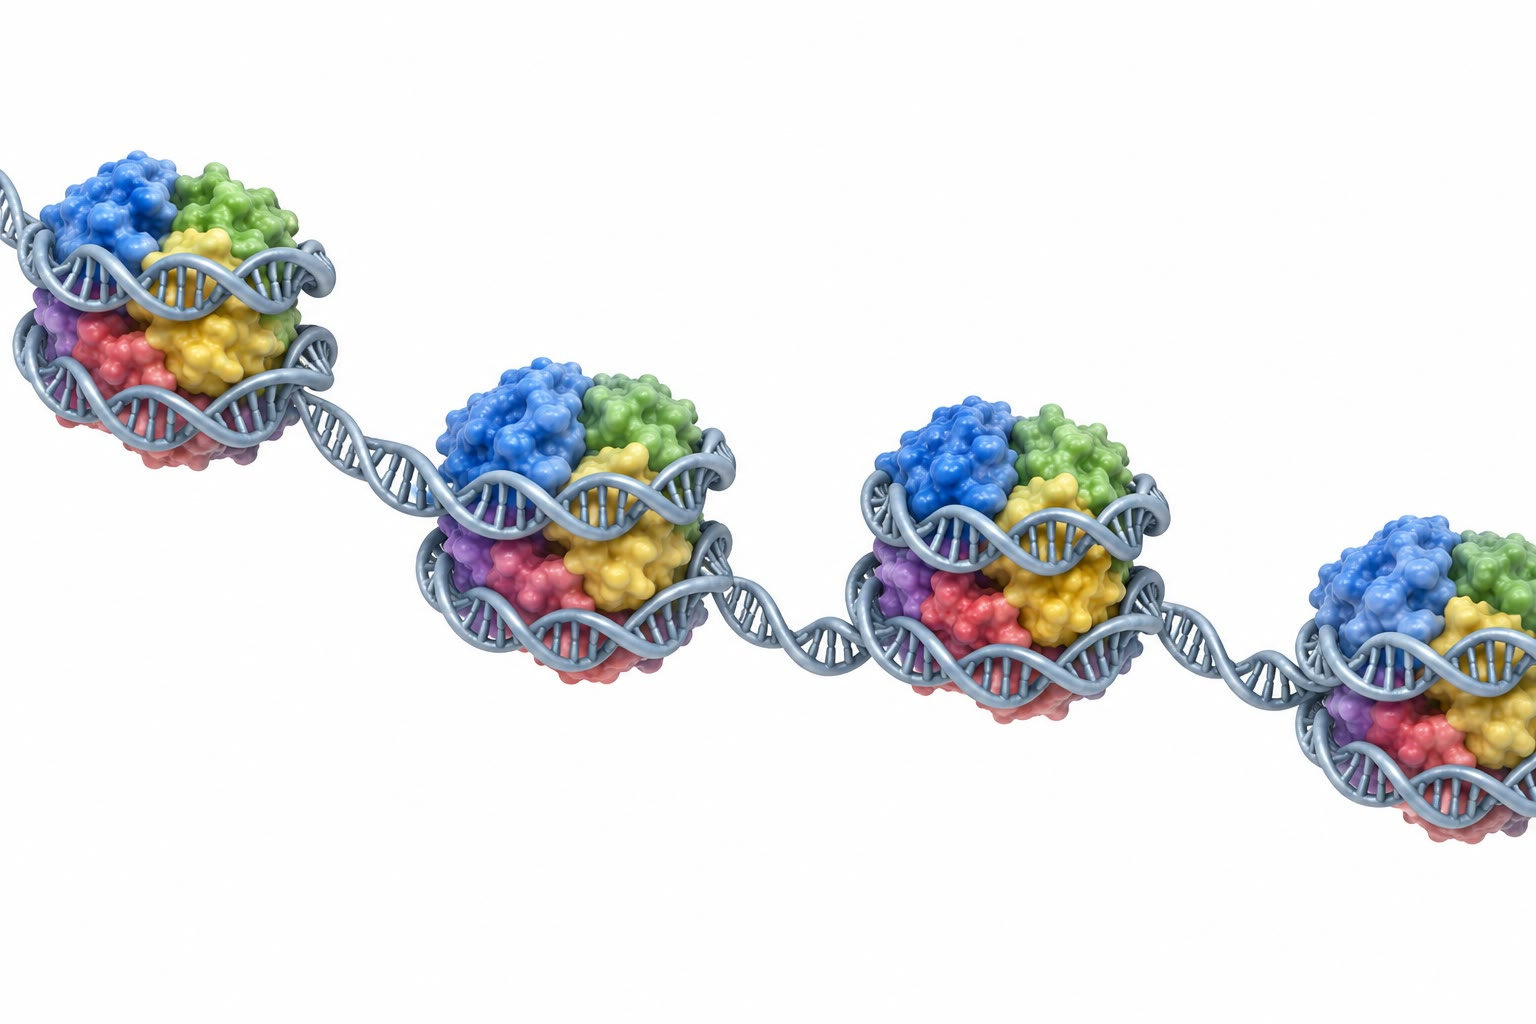
\includegraphics[width=0.6\linewidth]{images/book5/ai/b5-01-nucleosomes.jpg}

{\small \omterm{def:b3:chromatin-epigenetics:nucleosome}{الصبغين} على المقياس الجزيئي: اللولب المزدوج ملفوفًا حول لبوب
هستونية متعاقبة، وهي ``الخرزات على خيط'' التي كشفها سلّم النوكلياز.}
\end{omfigure}

\begin{proposition}[مستويات الرص]\label{prop:b3:chromatin-epigenetics:compaction}
\index{نسبة الرص}\index{عروة صبغينية}\index{نطاق مترابط طوبولوجيًا}
\emph{\omterm{prop:b3:chromatin-epigenetics:compaction}{نسبة الرص}} في بنية صبغينية هي طول DNA الذي تحتويه مقسومًا على
طول البنية. ويعطي اللف في ليف \qty{10}{nm} نسبة تقارب $6$: إذ تُضغط
\qty{68}{nm} من دورة \qty{200}{bp} في خرزة واحدة قطرها \qty{11}{nm}.
وفي النواة البينية لا يُلف الليف في ليف أغلظ منتظم، كما رسمته الكتب
طويلًا، بل يُطوى في \emph{عرى} تبلغ عشرات الكيلوقواعد إلى مئاتها
تُمسك عند قواعدها بمعقدات كوهيزين الحلقية وببروتين CTCF الرابط
لجزيء DNA؛ وتنتظم العرى في \emph{نطاقات مترابطة طوبولوجيًا} (TAD) يبلغ
حجم الواحد منها نحو ميغاقاعدة، تلتقي داخلها المورّثة بمنظماتها أكثر
بكثير مما تلتقي بأي شيء خارجها. أما الصبغي الانقسامي، وهو أشد
الحالات رصًا، فنسبة رصه قرب \num{10000}: إذ تُطوى \qty{4}{cm} من DNA
في صبغي بشري وسطي لتصير قضيبًا طوله \qty{4}{\micro m}.
\end{proposition}

\begin{example}[مترانِ في عشرة ميكرومترات]\label{ex:b3:chromatin-epigenetics:two-metres}
تضم النواة البشرية ثنائية الصيغة $6.4\times 10^{9}$ زوج قواعد. وعند
\qty{0.34}{nm} لكل زوج قواعد يكون ذلك \qty{2.2}{m} من اللولب المزدوج،
في نواة قطرها نحو \qty{10}{\micro m}. ويُرصّ ذلك في
$6.4\times 10^{9}/200 \approx 3.2\times 10^{7}$ \omterm{def:b3:chromatin-epigenetics:nucleosome}{جسيم نووي}، يحمل كل
منها نحو \qty{108}{kDa} من \omterm{def:b3:chromatin-epigenetics:nucleosome}{الهستون} مقابل \qty{96}{kDa} من DNA
(\qty{147}{bp} بوزن \qty{650}{Da} للزوج): فالنواة تحوي من \omterm{def:b3:chromatin-epigenetics:nucleosome}{الهستون}
كتلةً تقارب ما تحويه من DNA. أما DNA نفسه، إذا عُدّ أسطوانة قطرها
\qty{2}{nm}، فحجمه لا يتجاوز \qty{7}{\micro m^3}، أي نحو
\qty{1}{\%} من نواة كروية نصف قطرها \qty{5}{\micro m}؛ فمشكلة الرص
مشكلة تشابك ونفاذ، لا مشكلة حيّز.
\end{example}

\section{شيفرة الهستونات}

\begin{definition}[تعديلات الهستونات]\label{def:b3:chromatin-epigenetics:histone-code}
\index{شيفرة الهستونات}\index{أستلة}\index{مثيلة الهستونات}\index{كاتب}\index{قارئ}\index{ماحٍ}
تُعدَّل بقايا ذيول الهستونات تعديلًا تساهميًا: \emph{أستلة} الليزينات
(وهي تعادل شحنتها الموجبة فتُرخي قبضتها على DNA)، و\emph{مثيلة}
الليزينات والأرجينينات (زمرة ميثيل أو اثنتان أو ثلاث، بلا تغير في
الشحنة)، وفسفرة السيرينات، وأبيقنة الليزينات. ويُسمّى التعديل
\omterm{def:b3:chromatin-epigenetics:nucleosome}{بالهستون} والبقية والزمرة: فالعلامة H3K4me3 هي \omterm{def:b3:chromatin-epigenetics:nucleosome}{الهستون} H3، الليزين 4،
ثلاثي المثيلة؛ وH3K27ac هو H3 الليزين 27 مؤستلًا. و\emph{شيفرة
الهستونات} هي الارتباط بين توليفات العلامات وحالة المورّثة الكامنة
تحتها: H3K4me3 وH3K27ac عند المروّجات والمعزِّزات النشطة، وH3K36me3
على امتداد أجسام المورّثات المستنسخة، وH3K9me3 على \omterm{def:b3:chromatin-epigenetics:nucleosome}{الصبغين المتغاير}
البنيوي، وH3K27me3 على المورّثات المُسكتة أثناء التطور. والإنزيمات
التي تضيف علامة هي \emph{الكتبة} (ناقلات الأستيل الهستونية HAT،
وناقلات الميثيل)، والإنزيمات التي تزيلها هي \emph{المواحي} (نازعات
الأستيل الهستونية HDAC، ونازعات الميثيل)، والبروتينات التي ترتبط
بعلامة وتعمل بموجبها هي \emph{القرّاء}: إذ يرتبط \emph{النطاق البرومي}
بالليزين المؤستل، ويرتبط \emph{النطاق الكرومي} بالليزين الممثيل.
\end{definition}

\begin{proposition}[العلامات تُقرأ، لا تُحسّ فحسب]\label{prop:b3:chromatin-epigenetics:readers}
\index{HP1}\index{بوليكومب}\index{PRC2}\index{تريثوراكس}
تعمل \omterm{def:b3:chromatin-epigenetics:histone-code}{الأستلة} جزئيًا بالكهرباء الساكنة --- فالذيل المؤستل يمسك DNA
أقل شدة فينفتح الليف --- غير أن معظم العلامات تعمل باستدعاء القرّاء.
فالعلامة H3K9me3 يرتبط بها النطاق الكرومي من \emph{بروتين \omterm{def:b3:chromatin-epigenetics:nucleosome}{الصبغين المتغاير}
HP1}، الذي يتثنّى ويجسر بين جسيمين نوويين متجاورين ويستدعي ناقلة
الميثيل نفسها (SUV39H) التي تكتب H3K9me3 على \omterm{def:b3:chromatin-epigenetics:nucleosome}{الجسيم النووي} التالي:
فتنتشر العلامة على امتداد الليف حتى تلقى حدًّا، وترصّ ما تغطيه.
أما H3K27me3 فيكتبه \emph{معقّد بوليكومب الكابح 2} (PRC2، ووحدته
الحفّازة EZH2)، ويقرأه PRC1 الذي يؤبقن H2A ويرصّ الليف، والمعقّد
نفسه تحفزه العلامة التي يصنعها؛ وتكتب زمرة بروتينات
\emph{تريثوراكس} العلامة المضادة H3K4me3 وتُبقي مورّثات التطور
الخاصة بنمط خلوي بعينه مفتوحة. وكل عروة من هذا القبيل --- \omterm{def:b3:chromatin-epigenetics:histone-code}{قارئ}
يستدعي كاتبًا --- تغذية راجعة موجبة تتيح للحالة أن تصون نفسها متى
ترسخت، وهذا ما تحتاجه العلامة القابلة للتوريث.
\end{proposition}

\begin{omfigure}
\begin{tikzpicture}[every node/.style={font=\scriptsize}, >=stealth]
  % nucleosomes with tails
  \foreach \x in {0,2,4,6} { \draw[thick, omDef, fill=omDef!20] (\x,0) circle (0.45); \draw[omProp, thick] (\x,0.45) -- (\x,1.15); }
  % marks
  \fill[omThm] (2,1.15) circle (0.11); \fill[omThm] (4,1.15) circle (0.11);
  \fill[omMeth!80!black] (0,1.15) circle (0.11);
  \node[left] at (-0.5,1.15) {ac};
  \node[right, align=left] at (6.15,1.15) {me3};
  % HP1 reader
  \draw[thick, fill=omExo!30] (2.6,1.7) ellipse (0.5 and 0.25); \node at (2.6,1.7) {قارئ};
  \draw[thick, fill=omExo!30] (4.2,2.35) ellipse (0.55 and 0.25); \node at (4.2,2.35) {كاتب};
  \draw[->, thick] (2.9,1.9) -- (3.75,2.2);
  \draw[->, thick, omThm] (4.6,2.15) .. controls (5.6,2.0) and (6.1,1.8) .. (6.05,1.3);
  \node[right, align=left, font=\scriptsize] at (6.6,2.0) {ينتشر إلى الجسيم\\النووي التالي};
  \draw[->, thick, gray] (2.2,1.3) -- (2.45,1.5);
  % eraser
  \draw[thick, fill=omExo!30] (0.6,2.2) ellipse (0.5 and 0.25); \node at (0.6,2.2) {ماحٍ};
  \draw[->, thick, omMeth!80!black] (0.3,2.0) -- (0.05,1.35);
  % DNA
  \draw[very thick, omThm!70!black] (-0.9,-0.3) -- (-0.45,-0.05) (0.45,-0.05) -- (1.55,-0.05) (2.45,-0.05) -- (3.55,-0.05) (4.45,-0.05) -- (5.55,-0.05) (6.45,-0.05) -- (7.2,-0.3);
  \node[below, align=center] at (0,-0.6) {مفتوح: زمرة الأستيل\\تزيل شحنة};
  \node[below, align=center] at (5,-0.6) {مغلق: HP1 يقرأ H3K9me3،\\فيستدعي ميثيلاز K9};
\end{tikzpicture}

{\small منطق \omterm{def:b3:chromatin-epigenetics:histone-code}{الكاتب} \omterm{def:b3:chromatin-epigenetics:histone-code}{والقارئ} والماحي. \omterm{def:b3:chromatin-epigenetics:histone-code}{القارئ} المرتبط بعلامة على \omterm{def:b3:chromatin-epigenetics:nucleosome}{جسيم
نووي} يستدعي \omterm{def:b3:chromatin-epigenetics:histone-code}{الكاتب} الذي يضع العلامة نفسها على الجسيم التالي، فتنتشر
الحالة وتنسخ نفسها؛ والمواحي تعاكسها. زمر الأستيل (بالأخضر) تفتح
الليف، وH3K9me3 (بالأحمر) يغلقه.}
\end{omfigure}

\begin{method}[الترسيب المناعي للصبغين (ChIP)]\label{met:b3:chromatin-epigenetics:chip}
\index{ChIP}\index{ترسيب مناعي للصبغين}
لرسم موضع علامة أو بروتين على الجينوم: (1) تُشبك البروتينات بجزيء DNA في
الخلايا الحية بالفورمالدهيد؛ (2) يُقصّ \omterm{def:b3:chromatin-epigenetics:nucleosome}{الصبغين} إلى قطع من بضع مئات
من أزواج القواعد؛ (3) تُرسَّب القطع بجسم مضاد تجاه العلامة (وليكن
H3K27me3) مثبت على حبيبات؛ (4) تُعكس الشبكات ويُنقّى DNA؛ (5)
يُسلسل (ChIP-seq) وتُعدّ القراءات على امتداد الجينوم: فالذرى هي
المواضع التي كانت فيها العلامة. وتضبط عينةُ الدخل من DNA بلا جسم
مضاد مستوى الخلفية. أما التمييز فهو تمييز القطع، أي نحو \omterm{def:b3:chromatin-epigenetics:nucleosome}{جسيم نووي}
واحد.
\end{method}

\begin{remark}[شيفرة أم ارتباط]\label{rem:b3:chromatin-epigenetics:code}
لفظ ``الشيفرة'' يبالغ في الأمر. فكثير من العلامات نتائج للاستنساخ لا
أسباب له (H3K36me3 تضعه ناقلة ميثيل تسير مع البوليميراز)، وحذف \omterm{def:b3:chromatin-epigenetics:histone-code}{كاتب}
ما كثيرًا ما يغير التعبير أقل بكثير مما يوحي به توزع علامته. والمقرر
أن بضع علامات --- H3K9me3 وH3K27me3 \omterm{def:b3:chromatin-epigenetics:methylation}{ومثيلة DNA} أدناه --- تحمل إسكاتًا
ذاتي الانتشار يعمّر بعد زوال الإشارة التي أنشأته.
\end{remark}

\section{مثيلة DNA ونسخ العلامة}

\begin{definition}[مثيلة DNA]\label{def:b3:chromatin-epigenetics:methylation}
\index{مثيلة DNA}\index{CpG}\index{جزيرة CpG}\index{DNMT1}\index{مثيلة صيانة}\index{مثيلة مستجدة}
في الفقاريات تُضاف زمرة ميثيل إلى الكربون 5 من السيتوزين، ولا يكاد
ذلك يحدث إلا في ثنائي النوكليوتيد \emph{CpG} (سيتوزين يتبعه غوانين
على الطاق نفسه)، وهو متتالية متممة لنفسها، فثنائي CpG الممثيل يكون ممثيلًا
عادةً على الطاقين معًا. ونحو \qtyrange{70}{80}{\%} من CpG في الخلية
البشرية ممثيلة، والمروّجات الممثيلة صامتة: إذ تقرأ زمرَ الميثيل
بروتيناتٌ رابطة بثنائي CpG الممثيل (MeCP2 وMBD1--4) تستدعي HDAC وميثيلازات
H3K9، وتحجب عدة عوامل استنساخ حجبًا مباشرًا. والاستثناء هو
\emph{جزر CpG}، وهي قطع طولها نحو كيلوقاعدة، غنية بالقاعدتين G وC وبثنائيات CpG،
تقع عند مروّجات معظم مورّثات التدبير المنزلي وتبقى غير ممثيلة في
الخلايا السوية. وتكتب زمرة الميثيل \emph{ناقلات ميثيل DNA}: فالإنزيمان DNMT3A وDNMT3B تنفذان \emph{المثيلة المستجدة} للمواقع غير
الممثيلة، و\emph{DNMT1}، التي تفضّل CpG نصف ممثيل --- طاق ممثيل وآخر غير
ممثيل --- تنفذ \emph{مثيلة الصيانة} خلف شوكة التضاعف. أما الإزالة
فسلبية بالتضاعف من دون صيانة، أو فعالة بإنزيمات TET التي تؤكسد
5-ميثيل سيتوزين إلى 5-هيدروكسي ميثيل سيتوزين وما بعده حتى يستبدل به
إصلاحُ استئصال القاعدة سيتوزينًا عاديًا.
\end{definition}

\begin{example}[لماذا يفتقر الجينوم إلى CpG]\label{ex:b3:chromatin-epigenetics:cpg-deficit}
الجينوم البشري \qty{42}{\%} من G$+$C، فلو كانت القواعد مستقلة لورد
\omterm{def:b3:chromatin-epigenetics:methylation}{CpG} بتواتر $0.21\times 0.21 \approx 0.044$، أي نحو
$2.8\times 10^{8}$ مرة في الجينوم ثنائي الصيغة. والعدد المرصود نحو
$5.6\times 10^{7}$، أي خُمس ذلك. والسبب هو العلامة نفسها: فالسيتوزين
الممثيل إذا فقد زمرته الأمينية صار ثيمينًا، وهي قاعدة سوية لا يستطيع
الإصلاح أن يعدّها خطأً، في حين أن السيتوزين غير الممثيل ينزع أمينه
فيصير يوراسيلًا يُستأصل. وعبر الزمن التطوري تحولت \omterm{def:b3:chromatin-epigenetics:methylation}{CpG} الممثيلة إلى
TpG وCpA، ولم تحتفظ بثنائياتها إلا الجزر غير الممثيلة. فقد تركت العلامة
بصمتها في التسلسل نفسه.
\end{example}

\begin{theorem}[صيانة حالة المثيلة عبر الانقسامات]\label{thm:b3:chromatin-epigenetics:maintenance}
\index{ذاكرة لاجينية}\index{سلسلة ماركوف!المثيلة}
لنأخذ موقع \omterm{def:b3:chromatin-epigenetics:methylation}{CpG} واحدًا ونتابعه في سلالة من الخلايا. عند كل انقسام
يُمثيل سيتوزين الطاق الجديد باحتمال $\mu$ إذا كان سيتوزين الطاق
القالب ممثيلًا (كفاءة الصيانة)، وباحتمال $\delta$ إذا لم يكن (معدل
\omterm{def:b3:chromatin-epigenetics:methylation}{المثيلة المستجدة}). وليكن $p_{n}$ احتمال أن يكون الموقع ممثيلًا بعد
$n$ انقسامًا. عندئذٍ
\[
p_{n+1} = \mu\, p_{n} + \delta\,(1 - p_{n}),
\qquad
p_{n} = p^{*} + (p_{0} - p^{*})\,(\mu - \delta)^{n},
\qquad
p^{*} = \frac{\delta}{1 - \mu + \delta}.
\]
ينجرف كل موقع نحو التوازن $p^{*}$ نفسه مهما كانت حالته الابتدائية،
وتتلاشى ذاكرة الحالة الابتدائية تلاشيًا هندسيًا بنسبة $\mu - \delta$.
وتُذكر العلامة نحو $1/(1 - \mu + \delta)$ انقسامًا؛ ومن ثم فإن
الذاكرة الأمينة لأي \emph{فرق} بين موقعين تقتضي أن يكون $\mu$ قريبًا
جدًا من $1$ و$\delta$ قريبًا جدًا من $0$، أو أن تكون هناك تغذية راجعة
تجعل $\mu$ و$\delta$ تابعين لحالة الجوار.
\end{theorem}
\begin{proof}
التكرار هو قانون الاحتمال الكلي على حالتي القالب. وتحل نقطته الثابتة
$p^{*} = \mu p^{*} + \delta(1 -
p^{*})$، فينتج $p^{*}(1 - \mu + \delta) = \delta$. وبطرح معادلة النقطة الثابتة من
التكرار نجد $p_{n+1} - p^{*} = (\mu -
\delta)(p_{n} - p^{*})$، وهو ما يتكرر إلى الصيغة المغلقة. وبما أن
$0 \le \delta \le \mu \le 1$، فإن النسبة $\mu - \delta$ تقع في $[0,1]$
والانحراف يتقلص؛ وينتصف كل $\ln 2 / (-\ln(\mu -
\delta)) \approx \ln 2/(1 - \mu + \delta)$ انقسامًا حين يكون $\mu -
\delta$ قريبًا من $1$.
\end{proof}

\begin{example}[أرقام]\label{ex:b3:chromatin-epigenetics:maintenance-numbers}
القيم المقيسة في خلايا الثدييات هي $\mu \approx 0.99$ و
$\delta \approx 0.02$ لكل انقسام عند \omterm{def:b3:chromatin-epigenetics:methylation}{CpG} نمطي. ومن ثم $p^{*} =
0.02/0.03 \approx 0.67$، وهي قريبة من نسبة المثيلة على مستوى الجينوم،
و$\mu - \delta = 0.97$: فموقع ممثيل تمامًا متروك للآلية وحدها يقطع
نصف الطريق عائدًا إلى المتوسط بعد $\ln 2 /
0.03 \approx 23$ انقسامًا. فالمروّج المُسكت الذي يبقى صامتًا مئات
الانقسامات في عمر كامل يحتاج إذن إلى أكثر من \omterm{def:b3:chromatin-epigenetics:methylation}{DNMT1}: فقرّاء \omterm{def:b3:chromatin-epigenetics:methylation}{CpG}
الممثيل يستدعون مثيلة H3K9، وقرّاء H3K9 يستدعون DNMT3، حتى إن جزيرة
كثيفة العلامات ترفع $\mu$ الخاص بها نحو $1$ وتخفض $\delta$ المجاور
نحو $0$. وعلى العكس، فالخلية التي تفقد \omterm{def:b3:chromatin-epigenetics:methylation}{DNMT1} تفقد العلامة سلبيًا:
فمع $\mu = \delta = 0$ تنتصف نسبة الطاقات الممثيلة عند كل انقسام.
\end{example}

\begin{omfigure}
\begin{tikzpicture}[every node/.style={font=\scriptsize}, >=stealth]
  % left: replication scheme
  \begin{scope}
    \draw[very thick, omThm!70!black] (0,1.2) -- (2.4,1.2); \draw[very thick, omThm!70!black] (0,0.9) -- (2.4,0.9);
    \foreach \x in {0.5,1.2,1.9} { \fill[omDef] (\x,1.2) circle (0.09); \fill[omDef] (\x,0.9) circle (0.09); }
    \node[above] at (1.2,1.3) {الأصل: الطاقان ممثيلان};
    \draw[->, thick] (1.2,0.75) -- (1.2,0.15) node[midway, right] {التضاعف};
    \draw[very thick, omThm!70!black] (0,-0.1) -- (2.4,-0.1); \draw[very thick, gray] (0,-0.4) -- (2.4,-0.4);
    \foreach \x in {0.5,1.2,1.9} { \fill[omDef] (\x,-0.1) circle (0.09); \draw[omDef] (\x,-0.4) circle (0.09); }
    \node[left] at (-0.1,-0.25) {نصف ممثيل};
    \draw[->, thick] (1.2,-0.85) -- (1.2,-1.45) node[midway, right, align=left] {DNMT1، باحتمال $\mu$\\لكل موقع};
    \draw[very thick, omThm!70!black] (0,-1.7) -- (2.4,-1.7); \draw[very thick, gray] (0,-2.0) -- (2.4,-2.0);
    \foreach \x in {0.5,1.9} { \fill[omDef] (\x,-1.7) circle (0.09); \fill[omDef] (\x,-2.0) circle (0.09); }
    \fill[omDef] (1.2,-1.7) circle (0.09); \draw[omDef] (1.2,-2.0) circle (0.09);
    \node[below, align=center] at (1.2,-2.1) {استُعيدت، مع تفويت موقع:\\الطاق الجديد للبنت};
  \end{scope}
  % right: decay plot
  \begin{scope}[xshift=5.0cm, yshift=-2.3cm]
  \begin{axis}[
    width=6.6cm, height=4.6cm, axis lines=left,
    xmin=0, xmax=100, ymin=0, ymax=1.05,
    xlabel={الانقسامات $n$},
    xlabel style={font=\scriptsize, at={(axis description cs:0.5,-0.1)}, anchor=north},
    tick label style={font=\scriptsize}, xtick={0,25,50,75,100}, ytick={0,0.5,0.67,1},
    yticklabels={0,0.5,$p^{*}$,1}, clip=false,
  ]
  \addplot[very thick, omDef, domain=0:100, samples=60] {0.6667 + 0.3333*0.97^x};
  \addplot[very thick, omThm, domain=0:100, samples=60] {0.6667 - 0.6667*0.97^x};
  \addplot[dashed, gray, domain=0:100, samples=2] {0.6667};
  \addplot[thick, omMeth!80!black, domain=0:100, samples=60] {0.6667 + 0.3333*0.998^x};
  \node[font=\scriptsize] at (axis cs:-9,1.1) {$p_{n}$};
  \node[font=\scriptsize, omDef, anchor=south west] at (axis cs:45,0.82) {بداية ممثيلة، $\mu = 0.99$};
  \node[font=\scriptsize, omThm, anchor=north west] at (axis cs:50,0.30) {بداية غير ممثيلة};
  \node[font=\scriptsize, omMeth!80!black, anchor=south west] at (axis cs:30,1.02) {مع تغذية راجعة، $\mu = 0.999$};
  \end{axis}
  \end{scope}
\end{tikzpicture}

{\small يسارًا: \omterm{def:b3:chromatin-epigenetics:methylation}{مثيلة الصيانة}. بعد التضاعف يصير كل \omterm{def:b3:chromatin-epigenetics:methylation}{CpG} نصف ممثيل،
وينسخ \omterm{def:b3:chromatin-epigenetics:methylation}{DNMT1} العلامة على الطاق الجديد باحتمال $\mu$ لكل موقع. يمينًا:
مصير موقع عبر الانقسامات عند $\mu = 0.99$ و$\delta = 0.02$ (بالأزرق
من حالة ممثيلة، وبالأحمر من حالة غير ممثيلة) --- وكلاهما يتقارب إلى
$p^{*} = 0.67$ --- ثم موقع ترفع تغذيةُ جواره الراجعةُ $\mu$ فيه إلى
$0.999$ (بالأخضر).}
\end{omfigure}

\begin{method}[قراءة المثيلة: تسلسل البيسلفيت]\label{met:b3:chromatin-epigenetics:bisulfite}
\index{تسلسل البيسلفيت}
لا يرى التسلسل وحده زمرة الميثيل. عالِج DNA المفكوك ببيسلفيت
الصوديوم: فالسيتوزين غير الممثيل يُنزع أمينه فيصير يوراسيلًا يُقرأ
T بعد PCR، أما 5-ميثيل سيتوزين فمحمي ويبقى يُقرأ C. سلسِل DNA
المحوَّل وقارنه بالمرجع: فكل C بقي C كان ممثيلًا، وكل C صار T لم
يكن. وإذا أُجري ذلك على الجينوم كله (\omterm{met:b3:chromatin-epigenetics:bisulfite}{تسلسل البيسلفيت} للجينوم الكامل)
أعطى حالة المثيلة في كل واحد من $2.8\times 10^{7}$ موقع \omterm{def:b3:chromatin-epigenetics:methylation}{CpG} في
جينوم أحادي الصيغة بتمييز القاعدة الواحدة، بوصفها نسبة من خلايا
العينة.
\end{method}

\section{تعطيل X والبصم الجينومي}

\begin{definition}[تعطيل الصبغي X]\label{def:b3:chromatin-epigenetics:x-inactivation}
\index{تعطيل X}\index{جسم بار}\index{Xist}\index{معاوضة الجرعة}
في إناث الثدييات يُسكت أحد الصبغيين X في كل خلية جسدية إسكاتًا
استنساخيًا باكرًا في التطور، وهو ضرب من \emph{معاوضة الجرعة} يسوّي
التعبير عن المورّثات المرتبطة بالصبغي X بين الإناث XX والذكور XY. ويُرصّ
الصبغي المُسكت في جسم كثيف ملتصق بالغلاف النووي هو \emph{جسم بار}.
واختيار أي الصبغيين X يُسكت اختيار عشوائي في الجنين نفسه، ومتى وقع
ورثته نسيليًا كل ذرية تلك الخلية. ويبدأ التعطيل بالجزيء \emph{Xist}، وهو
RNA غير مشفِّر طوله \qty{17}{kb} يُستنسخ من مركز تعطيل X في الصبغي
الذي سيُسكت: فيغلّف ذلك الصبغي على الجانب نفسه، ويستدعي بوليكومب
(H3K27me3)، وبديل \omterm{def:b3:chromatin-epigenetics:nucleosome}{الهستون} macroH2A، وأخيرًا \omterm{def:b3:chromatin-epigenetics:methylation}{مثيلة DNA} للمروّجات،
ثم تُصان السكتة بعد ذلك من دون حاجة إلى Xist في كل انقسام. وينجو من
التعطيل نحو \qty{15}{\%} من المورّثات البشرية المرتبطة بالصبغي X، كليًا أو
جزئيًا.
\end{definition}

\begin{proof}[شواهد]
لاحظ بار وبرترام (1949) جسمًا كثيفًا في أنوية عصبونات القطط الإناث
دون الذكور. وبيّن أونو (1959) أنه صبغي X كامل متكاثف. وجمع ليون
(1961) القطع معًا: فإناث الفئران المتغايرة اللواقح لمورّثات لون
الفروة المرتبطة بالصبغي X لها فروة فسيفسائية من بقع يعبَّر في كل منها عن
أليل أو آخر، فكل بقعة نسيلة أُسكت فيها أحد الصبغيين X، وهو نفسه
دائمًا؛ وينطبق ذلك على البقع البرتقالية والسوداء في قطة السلحفاة أو
الكاليكو، التي مورّثة اللون البرتقالي فيها مرتبطة بالصبغي X، وعلى الغدد
العرقية الفسيفسائية عند النساء الحاملات لأليل طافر من مورّثة مرتبطة
بالصبغي X. والقط الكاليكو الذكر يكاد يكون دائمًا XXY.
\end{proof}

\begin{omfigure}
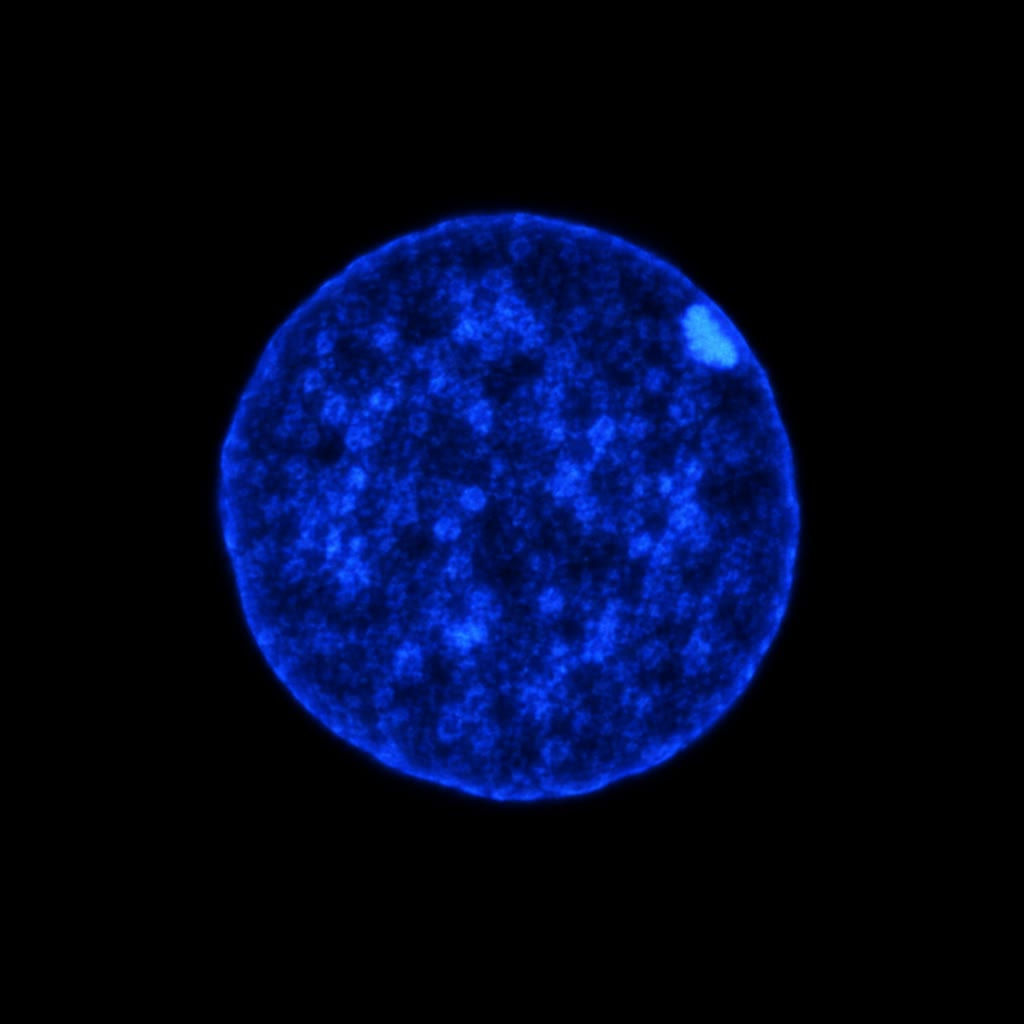
\includegraphics[width=0.42\linewidth]{images/book5/ai/b5-01-barr-body.jpg}\hspace{0.04\linewidth}
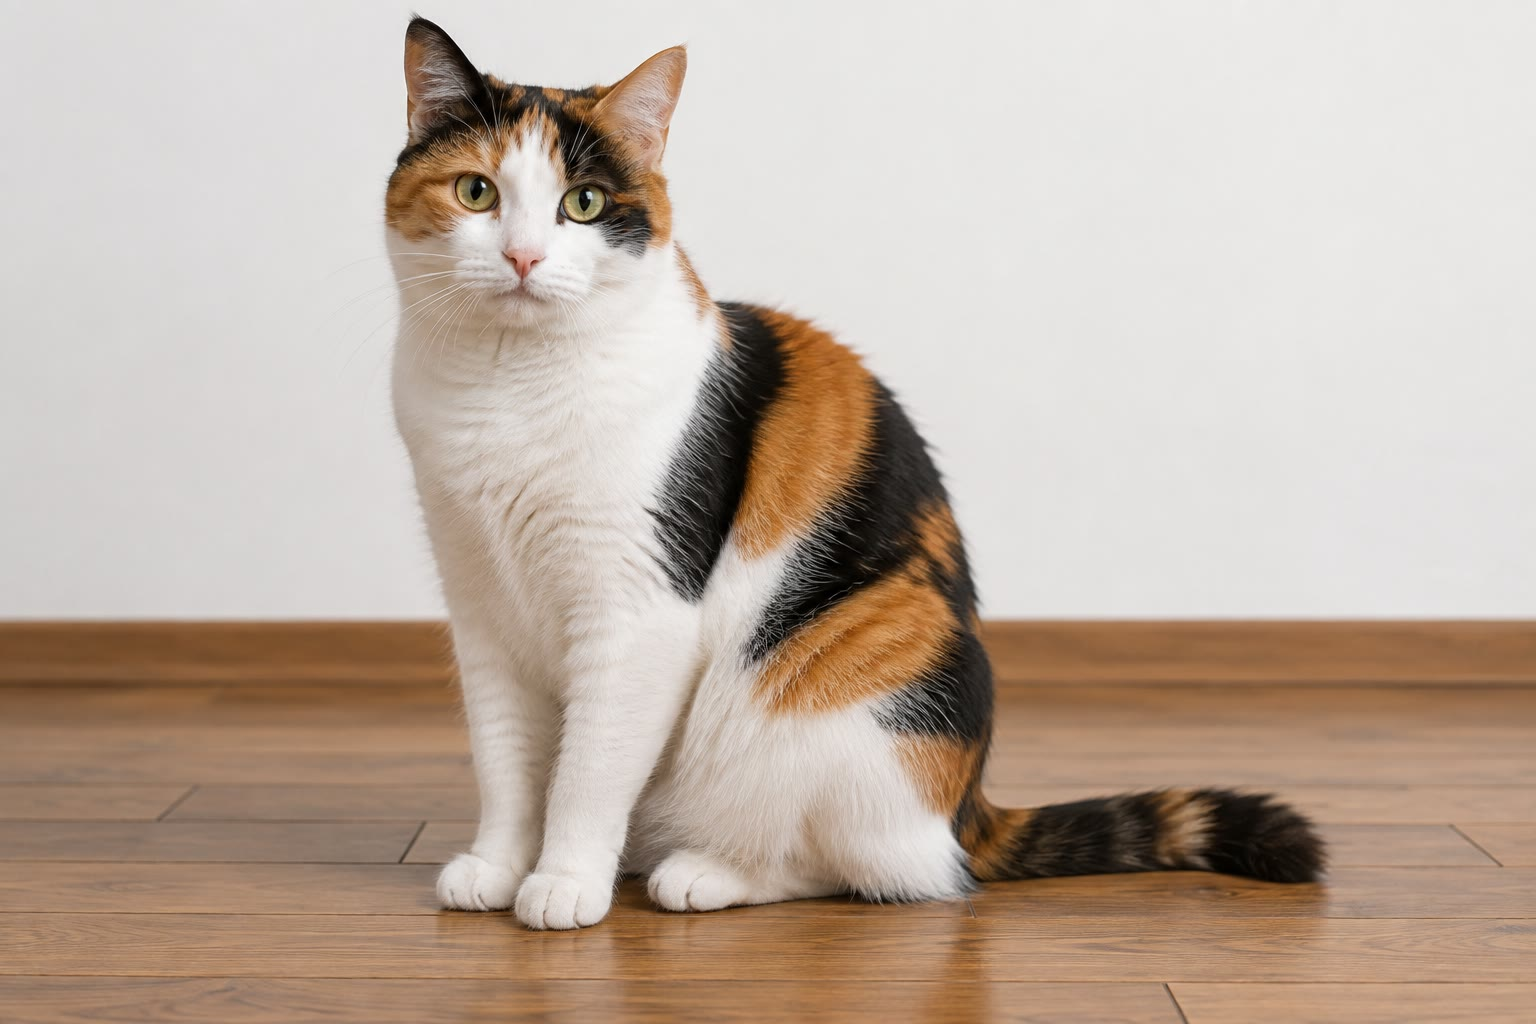
\includegraphics[width=0.5\linewidth]{images/book5/ai/b5-01-calico-cat.jpg}

{\small يسارًا: نواة أنثوية مصطبغة لجزيء DNA، وفيها الصبغي X المعطل
المرصوص --- \omterm{def:b3:chromatin-epigenetics:x-inactivation}{جسم بار} --- ملتصقًا بحافة النواة. يمينًا: قطة كاليكو.
كل بقعة برتقالية أو سوداء نسيلة من خلايا الجلد أسكتت الصبغي X نفسه؛
أما الأبيض فمورّثة تبقيع أخرى جسدية الصبغي.}
\end{omfigure}

\begin{definition}[البصم الجينومي]\label{def:b3:chromatin-epigenetics:imprinting}
\index{بصم جينومي}\index{منطقة التحكم بالبصم}\index{ثنائي الصيغة أحادي الأبوين}
تكون المورّثة \emph{مبصومة} حين لا يُعبَّر إلا عن أحد أليليها،
ويتوقف أيهما على الأب الذي جاء منه: فبعض المورّثات لا يُعبَّر عنها
إلا من النسخة الأبوية، وبعضها إلا من الأمومية. وللثدييات نحو
\numrange{100}{200} مورّثة مبصومة، متجمعة في عناقيد، يحكم كلًا منها
\emph{منطقة تحكم بالبصم} (ICR) ممثيلة على أحد الأليلين الأبويين دون
الآخر. وتُضبط المثيلة في السلالة الجنسية --- نمط في النطاف وآخر في
البيوض --- ثم تُمحى في الخلايا الجنسية للجيل التالي وتُضبط من جديد
وفق جنس ذلك الفرد. ومن ثم فالطفل الذي يتلقى نسختي صبغي من الأب نفسه
(\emph{ثنائي الصيغة أحادي الأبوين}) تكون عنده جرعة خاطئة من
المورّثات المبصومة عليه مع أن تسلسله سويّ تمامًا.
\end{definition}

\begin{proof}[شواهد]
صنع مكغراث وسولتر، وبالتوازي سوراني وبارتون ونوريس (1984)، لواقح
فئران تحمل نواتين أوليتين أموميتين، أو أبويتين، بنقل النوى الأولية
بين بيوض ملقحة. ولم يتطور أي من النوعين إلى نهاية الحمل، مع أن لكل
منهما طقمين كاملين من الصبغيات: فأجنّة النواتين الأموميتين كوّنت
جنينًا معقولًا بمشيمة رديئة، وأجنّة النواتين الأبويتين كوّنت مشيمة
كبيرة وبالكاد جنينًا. فالجينومان الأبويان ليسا متكافئين وكلاهما
مطلوب. وبيّن كاتاناتش وكيرك (1985) بثنائيات صيغة أحادية الأبوين
خاصة بصبغيات بعينها أن عدم التكافؤ محصور في مناطق بعينها من صبغيات
بعينها، وهي حيث وُجدت عناقيد البصم لاحقًا.
\end{proof}

\begin{example}[عنقود \emph{Igf2}--\emph{H19}]\label{ex:b3:chromatin-epigenetics:igf2}
يُعبَّر عن \emph{Igf2}، وهو عامل نمو جنيني، من الأليل الأبوي؛ ويُعبَّر
عن جاره \emph{H19}، وهو RNA غير مشفِّر، من الأمومي. وبينهما تقع ICR،
وخلف \emph{H19} تقع مجموعة معزِّزات مشتركة. فعلى الصبغي الأمومي تكون
ICR غير ممثيلة وترتبط بالبروتين CTCF الذي يعمل عازلًا: فتبلغ المعزِّزات
\emph{H19} ولا تبلغ \emph{Igf2}. وعلى الصبغي الأبوي تكون ICR ممثيلة
(ضُبطت في النطفة)، فلا يستطيع CTCF الارتباط، وتمتد المعزِّزات عبرها
إلى \emph{Igf2}؛ كما تنتشر المثيلة فتُسكت مروّج \emph{H19}. فعلامة
واحدة، ضُبطت في سلالة جنسية واحدة، تقرر مصير المورّثتين معًا.
\end{example}

\begin{omfigure}
\begin{tikzpicture}[every node/.style={font=\scriptsize}, >=stealth]
  \foreach \yy/\lab/\ctcf in {1.6/{الصبغي الأمومي}/1, -0.6/{الصبغي الأبوي}/0} {
    \draw[very thick, gray] (0,\yy) -- (9.4,\yy);
    \node[left, align=right] at (-0.15,\yy) {\lab};
    \draw[thick, fill=omDef!25] (1.0,\yy-0.2) rectangle (2.6,\yy+0.2); \node at (1.8,\yy) {\emph{Igf2}};
    \draw[thick, fill=omProp!30] (4.2,\yy-0.2) rectangle (5.2,\yy+0.2); \node at (4.7,\yy) {ICR};
    \draw[thick, fill=omDef!25] (6.2,\yy-0.2) rectangle (7.4,\yy+0.2); \node at (6.8,\yy) {\emph{H19}};
    \foreach \x in {8.4,8.8,9.2} \fill[omMeth!70!black] (\x,\yy) circle (0.12);
    \node[right] at (9.55,\yy) {معزِّزات};
  }
  % maternal: CTCF bound, enhancer -> H19
  \draw[thick, fill=omExo!35] (4.7,2.15) ellipse (0.45 and 0.22); \node at (4.7,2.15) {CTCF};
  \draw[->, thick, omMeth!70!black] (8.4,1.85) .. controls (7.8,2.5) and (7.2,2.5) .. (6.8,1.85);
  \node[above] at (7.6,2.35) {مفتوح};
  \draw[thick, omThm] (5.3,2.3) -- (5.3,0.9); \node[omThm, below] at (5.3,0.9) {عازل};
  \node[omThm, above=1.0cm, align=center, font=\scriptsize] at (1.8,1.8) {\emph{Igf2} صامت};
  % paternal: ICR methylated
  \foreach \x in {4.35,4.6,4.85,5.1} \fill[omThm] (\x,-0.95) circle (0.08);
  \node[below, align=center] at (4.7,-1.05) {ممثيلة:\\لا CTCF};
  \draw[->, thick, omMeth!70!black] (8.4,-0.35) .. controls (6.5,0.6) and (3.5,0.6) .. (1.8,-0.35);
  \node[above] at (3.3,0.2) {مفتوح};
  \foreach \x in {6.4,6.7,7.0,7.2} \fill[omThm] (\x,-0.95) circle (0.08);
  \node[below] at (6.8,-1.05) {مُسكت};
\end{tikzpicture}

{\small البصم عند \emph{Igf2}--\emph{H19}. الأليل الأمومي: ICR غير
الممثيلة ترتبط بالبروتين CTCF العازل، فلا تنشّط المعزِّزات التالية إلا
\emph{H19}. الأليل الأبوي: مُثيلت ICR في النطفة، فلا يستطيع CTCF
الارتباط، وتبلغ المعزِّزات \emph{Igf2}، وتُسكت المثيلة \emph{H19}.}
\end{omfigure}

\begin{example}[برادر--فيلي وأنجلمان]\label{ex:b3:chromatin-epigenetics:pws}
الحذف نفسه، وقدره نحو \qty{5}{Mb} من الصبغي 15 (المنطقة
15q11--q13)، يسبب \emph{متلازمة برادر--فيلي} --- ضعف المقوية العضلية
عند الولادة، ثم شره لا يُشبع وبدانة --- حين يقع على الصبغي الأبوي،
ويسبب \emph{متلازمة أنجلمان} --- إعاقة ذهنية شديدة وغياب الكلام
وهيئة مرحة ونوب اختلاجية --- حين يقع على الأمومي. فالمنطقة تحمل
مورّثات يُعبَّر عنها أبويًا (\emph{SNRPN} وعنقودًا من RNA صغيرة)
تُفقد نسختها الفاعلة الوحيدة في الحالة الأولى، وتحمل \emph{UBE3A}
المعبَّر عنها أموميًا، وهي المفقودة في الثانية. كما أن ثنائي الصيغة
الأمومي أحادي الأبوين للصبغي 15، بلا أي حذف، يعطي برادر--فيلي أيضًا:
نسختان أموميتان، صامتتان للمورّثات الأبوية.
\end{example}

\begin{remark}[لماذا البصم أصلًا]\label{rem:b3:chromatin-epigenetics:kinship}
المورّثات المبصومة غنية بالتحكم في نمو الجنين وفي نقل المغذيات عبر
المشيمة، وتميل المورّثات المعبَّر عنها أبويًا (\emph{Igf2} و
\emph{Peg3}) إلى تعزيز النمو، والمعبَّر عنها أموميًا (\emph{H19} و
\emph{Igf2r} و\emph{Cdkn1c}) إلى كبحه. وتقرأ \emph{نظرية القرابة}
ذلك تنازعًا: فمورّثات الأب تكسب من انتزاع المزيد من أمّ قد تحمل
لاحقًا ذرية ذكور آخرين، ومورّثات الأم تكسب من توزيع المؤونة على
بطونها كلها. والبصم يقع في الثدييات المشيمية وفي النباتات الزهرية،
التي تغذي الأمُّ سويداءَها كذلك، ولا يقع في الطيور ولا الزواحف، وهو
ما تتنبأ به النظرية.
\end{remark}

\section{الوراثة اللاجينية وحدودها}

\begin{definition}[علم اللاجينات]\label{def:b3:chromatin-epigenetics:epigenetics}
\index{علم اللاجينات}\index{أليل لاجيني}\index{إعادة البرمجة}
\emph{علم اللاجينات} هو دراسة التغيرات القابلة للتوريث في نشاط
المورّثات من غير أن تكون تغيرات في تسلسل DNA: حالات تحملها \omterm{def:b3:chromatin-epigenetics:methylation}{مثيلة DNA}
أو علامات الهستونات أو دارات عوامل استنساخ ذاتية الإدامة، وتُنسخ عبر
انقسام الخلية. وأليلان متطابقا التسلسل مختلفا الحالة اللاجينية
المستقرة هما \emph{أليلان لاجينيان}. والتوريث عبر الانقسام الفتيلي هو
القاعدة، وهو ما يُبقي الخلية المتمايزة متمايزة. أما التوريث عبر
الانقسام المنصّف، من الوالد إلى الخلف، فهو الاستثناء في الثدييات، لأن
العلامات تُمحى في موجتي \emph{إعادة برمجة}: في الخلايا الجنسية
البدئية، حيث تُمسح البصمات ومعظم المثيلة ثم تُضبط من جديد وفق الجنس،
ثم مرة أخرى في اللاقحة والجنين الباكر، حيث يُنزع الميثيل فعالًا من
الجينوم الأبوي بإنزيم TET3 ومن الأمومي سلبيًا، قبل أن ترسي DNMT3 أنماط
الجنين نفسه.
\end{definition}

\begin{example}[فأر الأغوتي الأصفر القابل للحياة]\label{ex:b3:chromatin-epigenetics:agouti}
في الأليل $A^{vy}$ اندس ناقل رجعي أعلى مورّثة لون الفروة
\emph{agouti}. فحيث يكون مروّج الناقل غير ممثيل يقود \emph{agouti}
باستمرار في كل خلية؛ فيكون الفأر أصفر بدينًا مهيّأً للسكري. وحيث
يكون ممثيلًا تتبع المورّثة تحكمها الطبيعي ويكون الفأر بنيًا
(``شبيه الأغوتي''). وتتوزع صغار البطن الواحدة المتطابقة وراثيًا على
الطيف كله، وللأم الصفراء صغار صفر أكثر مما للبنية: \omterm{def:b3:chromatin-epigenetics:epigenetics}{فالأليل اللاجيني}
لا يُمحى تمامًا عبر السلالة الجنسية الأمومية. وقد أطعم واترلاند
وجيرتل (2003) أمهات $A^{vy}$ الحوامل غذاءً غنيًا بواهبات الميثيل
(الفولات وفيتامين B\textsubscript{12} والكولين والبيتائين) فأزاحا
فراء الصغار نحو البني. فبيئة جيل واحد ضبطت علامة حملها الجيل التالي.
\end{example}

\begin{omfigure}
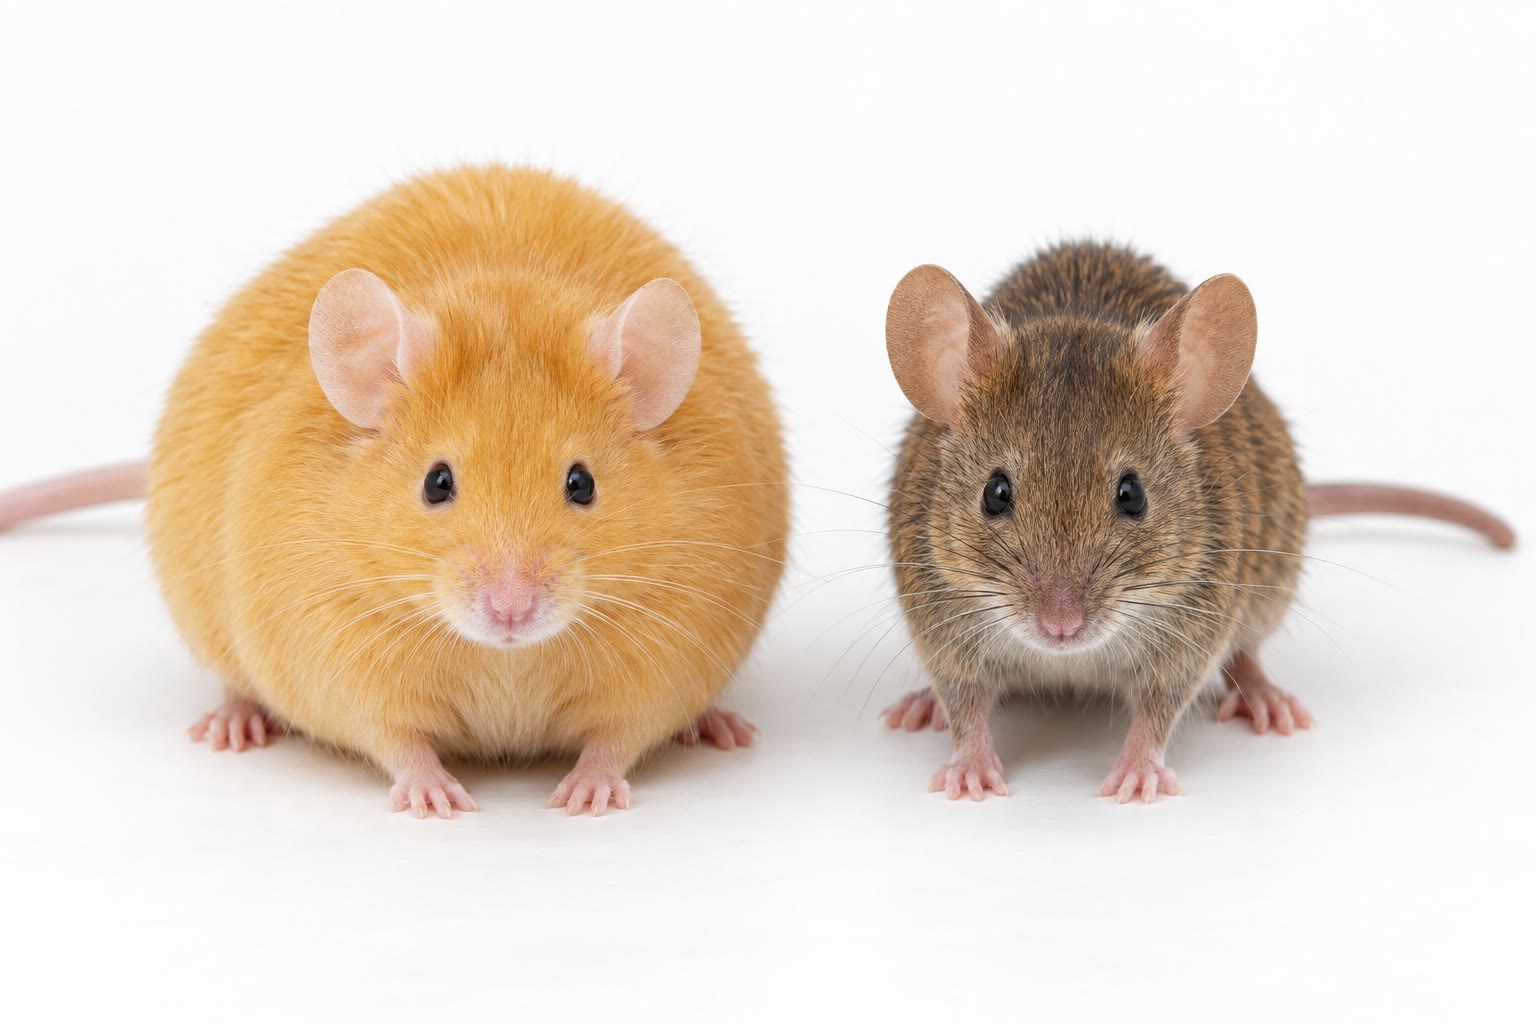
\includegraphics[width=0.62\linewidth]{images/book5/ai/b5-01-agouti-mice.jpg}

{\small صغيران من بطن $A^{vy}$ واحدة بالنمط الوراثي نفسه: فأر أصفر
بدين لم يُمثيل فيه الناقل الواقع أعلى \emph{agouti}، وفأر بني شبيه
بالأغوتي مُثيل فيه.}
\end{omfigure}

\begin{proposition}[أين توجد الحالات اللاجينية القابلة للتوريث]\label{prop:b3:chromatin-epigenetics:examples}
\index{تنوع أثر الموضع}\index{الإرباع}\index{الطفرة الجانبية}
ثلاث منظومات مدروسة جيدًا تجسّد الآليات السابقة.
\emph{\omterm{prop:b3:chromatin-epigenetics:examples}{تنوع أثر الموضع}} في \emph{Drosophila}: مورّثة نقلتها إعادة
ترتيب صبغية إلى جوار \omterm{def:b3:chromatin-epigenetics:nucleosome}{صبغين متغاير} تُسكت في بعض الخلايا دون بعض،
فتعطي عينًا مبقعة؛ كل بقعة نسيلة، والإسكات ينتشر من \omterm{def:b3:chromatin-epigenetics:nucleosome}{الصبغين المتغاير}
بعروة HP1، والمورّثات التي تكبح طفرتُها التنوعَ (مورّثات
\emph{Su(var)}) هي HP1 وناقلة ميثيل H3K9.
و\emph{الإرباع} في \emph{Arabidopsis}: أسابيع من برد الشتاء تُسكت
كابح الإزهار \emph{FLC} بالعلامة H3K27me3 الذي يضعه بوليكومب، وتصمد السكتة
شهور النمو الربيعي وآلاف الانقسامات الخلوية، وتُصفَّر في كل جيل حتى
يلزم كل نبتة أن تعيش شتاءها الخاص. و\emph{\omterm{prop:b3:chromatin-epigenetics:examples}{الطفرة الجانبية}} في
الذرة: أليل من مورّثة الصباغ \emph{b1}، إذا لقي أليلًا آخر بعينه في
متغاير اللواقح، حوّله إلى حالته الصامتة، ونقل الأليلُ المحوَّل
الحالةَ إلى ذريته أجيالًا، عبر مثيلة توجهها RNA صغيرة يتناولها
\cref{ch:b3:rna-regulation}. والتوريث في كل حالة انقسامي فتيلي
ومتين؛ أما الانتقال عبر الأجيال فإما أن يُصفَّر فعالًا (في النبات)
وإما أن يكون راشحًا جزئيًا (في الفئران).
\end{proposition}

\begin{remark}[حدود الدعاوى العابرة للأجيال]\label{rem:b3:chromatin-epigenetics:limits}
الدعوى بأن مجاعة جدٍّ أو كربه ``يُورَّث لاجينيًا'' إلى الأحفاد من
البشر شائعة وغير مبرهنة في معظمها. فبين علامة جسدية وحفيدٍ موجتا
محو، والمورّثات المبصومة وقليل من النواقل هي الناجيات الموثقة الوحيدة
من المحو في الثدييات، وفي الأتراب البشرية يصعب فصل أثر البيئة
المشتركة وأثر البيئة الرحمية وأثر الفروق الوراثية عن علامة محمولة في
السلالة الجنسية. أما الحالات المبرهنة --- $A^{vy}$، وبعض الأليلات
اللاجينية المرتبطة بالنواقل، والحالات التي تتوسطها RNA في الديدان
والنبات --- فحقيقية ومفهومة جزيئيًا وضيقة. ومبرهنة هذا الفصل تقول
لماذا: فمن دون تغذية راجعة تدفع $\mu$ إلى $1$ تنسى العلامة نفسها في
بضع عشرات من الانقسامات، وتضيف السلالة الجنسية تصفيرًا فعالًا فوق ذلك.
\end{remark}

\section{تمارين}

\begin{exercise}[$\star$]\label{exo:b3:chromatin-epigenetics:1}
اذكر تركيب \omterm{def:b3:chromatin-epigenetics:nucleosome}{الجسيم النووي} اللبّي، وطول DNA الذي يربطه، وطول الوصلة
النمطي. ولماذا أعطى هضم \omterm{def:b3:chromatin-epigenetics:nucleosome}{الصبغين} بالنوكلياز سلّمًا من القطع بدل لطخة
متصلة؟
\end{exercise}

\begin{exercise}[$\star$]\label{exo:b3:chromatin-epigenetics:2}
لجينوم ضفدع $3.0\times 10^{9}$ زوج قواعد في الطقم الأحادي. كم جسيمًا
نوويًا تحوي نواة ثنائية الصيغة، إذا كانت الدورة \qty{190}{bp}، وكم
يبلغ طول DNA فيها؟
\end{exercise}

\begin{exercise}[$\star$]\label{exo:b3:chromatin-epigenetics:3}
فُكّ رموز H3K27me3 وH4K16ac وH3S10ph. وقل في كل منها هل يقترن \omterm{def:b3:chromatin-epigenetics:nucleosome}{بصبغين}
نشط أم صامت، وسمِّ قارئًا للأولى.
\end{exercise}

\begin{exercise}[$\star$]\label{exo:b3:chromatin-epigenetics:4}
فسّر لماذا تكون قطة الكاليكو أنثى دائمًا تقريبًا، وما الذي يجب أن
يكون عليه الكاليكو الذكر.
\end{exercise}

\begin{exercise}[$\star\star$]\label{exo:b3:chromatin-epigenetics:5}
احسب نسبة رص ليف \qty{10}{nm} من أرقام
\cref{def:b3:chromatin-epigenetics:nucleosome} (الدورة \qty{200}{bp}،
والخرزة \qty{11}{nm})، والنسبة اللازمة لإدخال \qty{4}{cm} من DNA
لصبغي بشري وسطي في صبيغية انقسامية طولها
\qty{4}{\micro m}. بأي عامل إضافي يجب أن يُطوى الليف؟
\end{exercise}

\begin{exercise}[$\star\star$]\label{exo:b3:chromatin-epigenetics:6}
في نموذج \cref{thm:b3:chromatin-epigenetics:maintenance} عند
$\mu = 0.98$ و$\delta = 0.01$، أوجد $p^{*}$ وعدد الانقسامات التي
يفقد بعدها موقع بدأ ممثيلًا نصف فائضه فوق $p^{*}$. وأعد ذلك عند
$\mu = 0.999$ و$\delta = 0.001$.
\end{exercise}

\begin{exercise}[$\star\star$]\label{exo:b3:chromatin-epigenetics:7}
أعطت تجربة ChIP-seq على خلايا كبدية ذروة H3K4me3 وذروة H3K27ac عند
مروّج المورّثة $A$، ونطاقًا عريضًا من H3K27me3 فوق المورّثة $B$،
وH3K9me3 فوق المورّثة $C$. تنبأ بالحالة الاستنساخية لكل منها، وقل
أيّ المورّثتين $B$ و$C$ أرجح أن تُفتح في نمط خلوي آخر ولماذا.
\end{exercise}

\begin{exercise}[$\star\star$]\label{exo:b3:chromatin-epigenetics:8}
امرأة تحمل حذفًا لمنطقة \emph{UBE3A} على أحد الصبغيين 15 وهي سليمة.
وكان أبوها يحمل الحذف نفسه وكان سليمًا أيضًا. ما المتلازمة، إن وُجدت،
التي يتهدد كلًا من أبنائها خطرُها، وبأي احتمال؟ وماذا لو كان الحذف
قد جاءها من أمها؟
\end{exercise}

\begin{exercise}[$\star\star$]\label{exo:b3:chromatin-epigenetics:9}
تنبأ بنتيجة حذف مورّثة \emph{\omterm{def:b3:chromatin-epigenetics:x-inactivation}{Xist}} من أحد الصبغيين X في جنين فأرة؛
ثم من كليهما. وتنبأ بما يفعله مورثٌ نقيل من \emph{\omterm{def:b3:chromatin-epigenetics:x-inactivation}{Xist}} أُدخل في
صبغي جسدي بذلك الصبغي.
\end{exercise}

\begin{exercise}[$\star\star\star$]\label{exo:b3:chromatin-epigenetics:10}
فسّر، مستعينًا بما في \cref{ex:b3:chromatin-epigenetics:cpg-deficit}،
لماذا احتفظت جزر \omterm{def:b3:chromatin-epigenetics:methylation}{CpG} بثنائياتها بينما فقد سائر الجينوم أربعة أخماسها،
وما الذي يعنيه ذلك عن حالة مثيلة الجزر في السلالة الجنسية عبر الزمن
التطوري. ولماذا تسقط الحجة في مورّثة لا تُمثيل إلا في الكبد؟
\end{exercise}

\begin{exercise}[$\star\star\star$]\label{exo:b3:chromatin-epigenetics:11}
بيّن، باستعمال عروة \omterm{def:b3:chromatin-epigenetics:histone-code}{الكاتب} \omterm{def:b3:chromatin-epigenetics:histone-code}{والقارئ} في
\cref{prop:b3:chromatin-epigenetics:readers}، كيف يمكن لنطاق من
H3K9me3 أن يكون مستقرًا عبر التضاعف مع أن كل انقسام يخفف الهستونات
المعلَّمة إلى النصف بأخرى جديدة غير معلَّمة. وما الذي يحدد أين يتوقف
النطاق عن الانتشار؟ واقترح تجربة لاختبار تفسيرك.
\end{exercise}

\begin{exercise}[$\star\star\star$]\label{exo:b3:chromatin-epigenetics:12}
تقرر دراسةٌ أن لأحفاد من عاشوا مجاعةً مثيلةً متبدلة عند مورّثة نمو
وكتلةً جسمية أعلى. عدّد التفسيرات البديلة التي يجب استبعادها قبل
استنتاج أن علامة مثيلة انتقلت عبر السلالة الجنسية، وقل أي تجربة في
الفئران تحسم المسألة.
\end{exercise}

\section{مسألة: ذاكرة مورّثة مُسكتة}

\begin{problem}[{مسألة نهاية الأسبوع --- جينوم بشري مرصوص في نواته،
وعلامة مثيلة متابَعة عبر الانقسامات، وقطة كاليكو مقروءة خريطةً
نسيلية، وأمراض منطقة مبصومة معدودة، وتنتهي إلى عدد الانقسامات التي
تنجو فيها العلامة بلا تغذية راجعة وإلى حجم جمهرة الخلايا التي اختارت
صبغيها X}]
\label{pb:b3:chromatin-epigenetics:1}
معطيات: النواة البشرية ثنائية الصيغة تضم $6.4\times 10^{9}$ زوج
قواعد، بمعدل \qty{0.34}{nm} و\qty{650}{Da} للزوج؛ ودورة \omterm{def:b3:chromatin-epigenetics:nucleosome}{الجسيم النووي}
\qty{200}{bp}، وكتلة ثماني الهستونات \qty{108}{kDa}، والجسيم اللبّي
قرص قطره \qty{11}{nm} وثخنه \qty{5.5}{nm}. والنواة كرة قطرها
\qty{10}{\micro m}. والجينوم \qty{42}{\%} من G$+$C. والمثيلة عند
\omterm{def:b3:chromatin-epigenetics:methylation}{CpG} عادي: $\mu = 0.99$ و$\delta = 0.02$ لكل انقسام.

\medskip
\noindent\textbf{الجزء الأول --- الرصّ.}
\begin{enumerate}
  \item احسب طول DNA الكلي في النواة وعدد الجسيمات النووية.
  \item احسب كتلة \omterm{def:b3:chromatin-epigenetics:nucleosome}{الهستون} الكلية (ثمانيات فقط) وكتلة DNA،
        بالبيكوغرام ($\qty{1}{Da} = \qty{1.66e-24}{g}$).
  \item احسب حجم النواة والحجم الكلي للجسيمات اللبّية، معدودةً
        أسطوانات. ما نسبة ما تملؤه من النواة؟
  \item لو صُفّت الجسيمات النووية طرفًا إلى طرف ليفًا قطره
        \qty{10}{nm}، فكم يبلغ طول الليف، وما \omterm{prop:b3:chromatin-epigenetics:compaction}{نسبة الرص} قياسًا إلى
        DNA العاري؟
  \item يُطوى الليف في عرى طول الواحدة \qty{200}{kb} تثبتها كوهيزين.
        كم عروة، وكم جسيمًا نوويًا في العروة الواحدة؟
  \item بفرض الاستقلال، كم ثنائي نوكليوتيد \omterm{def:b3:chromatin-epigenetics:methylation}{CpG} يحوي الجينوم ثنائي
        الصيغة؟ والعدد المرصود $5.6\times 10^{7}$. ما النسبة
        المفقودة، وبأي آلية طفرية؟
\end{enumerate}

\medskip
\noindent\textbf{الجزء الثاني --- علامة عبر الانقسامات.}
\begin{enumerate}[resume]
  \item اكتب علاقة التكرار في $p_{n}$ واحسب $p^{*}$.
  \item موقع \omterm{def:b3:chromatin-epigenetics:methylation}{CpG} في مروّج ممثيل تمامًا عند $n = 0$. احسب $p_{n}$ بعد
        $10$ و$50$ و$200$ انقسام.
  \item بعد كم انقسامًا ينتصف الفائض $p_{n} - p^{*}$؟ والخلية الجذعية
        النسيجية تنقسم نحو مرة في الأسبوع: كم سنة ذلك؟
  \item يثبط دواءٌ \omterm{def:b3:chromatin-epigenetics:methylation}{DNMT1} تثبيطًا تامًا ($\mu = 0$) ويثبط DNMT3 كذلك
        ($\delta = 0$). بيّن أن نسبة الطاقات الممثيلة في الجمهرة
        تنتصف عند كل انقسام، وأوجد عدد الانقسامات اللازمة لخفض مثيلة
        \qty{80}{\%} دون \qty{5}{\%}.
  \item في جزيرة مُسكتة يستدعي قرّاء \omterm{def:b3:chromatin-epigenetics:methylation}{CpG} الممثيل مثيلة H3K9، التي
        تستدعي DNMT3، حتى يصير داخل الجزيرة
        $\mu = 0.9995$ و$\delta = 0.0005$. أعد حساب عمر النصف
        للفائض، بالانقسامات وبالسنين عند انقسام واحد في الأسبوع.
  \item فسّر في جملة واحدة لماذا تكون نتيجة السؤال 11 لا نتيجة
        السؤال 9 هي ما تقتضيه مورّثة مُسكتة مدى العمر، وأي ترتيب
        جزيئي ينتجها.
\end{enumerate}

\medskip
\noindent\textbf{الجزء الثالث --- خريطة الكاليكو.}
\begin{enumerate}[resume]
  \item قطة متغايرة اللواقح لمورّثة اللون البرتقالي المرتبطة بالصبغي X.
        فسّر لماذا لفروتها بقع برتقالية وسوداء، وما الذي تمثله
        البقعة الواحدة.
  \item وقع \omterm{def:b3:chromatin-epigenetics:x-inactivation}{تعطيل X} حين كان عدد الخلايا المقدَّر لها أن تكوّن الجلد
        $N$، واختارت كل منها صبغي X عشوائيًا. ما احتمال أن تختار
        الخلايا $N$ كلها الصبغي نفسه فتعطي قطة أحادية اللون؟
  \item لم توثَّق قطة متغايرة اللواقح أحادية اللون بين ما لعله مليار
        قطة؛ خذ الاحتمال $10^{-9}$ وقدّر $N$.
  \item مساحة جلد القطة نحو \qty{0.3}{m^2} ومتوسط بقعها
        \qty{15}{cm^2}. قدّر عدد البقع، وفسّر لماذا يفوق $N$.
  \item القط XXY كاليكو أيضًا. كم \omterm{def:b3:chromatin-epigenetics:x-inactivation}{جسم بار} تُظهر خلاياه؟ وكم في أنثى
        XXX وفي ذكر XY؟
  \item المورّثة الناجية من التعطيل حاضرة بنسختين فاعلتين في الإناث
        وبنسخة واحدة في الذكور. أعطِ سببًا واحدًا لاحتمال التسامح مع
        هذه النجاة وحالةً واحدة تكون فيها ذات أثر.
\end{enumerate}

\medskip
\noindent\textbf{الجزء الرابع --- الصبغي 15.}
\begin{enumerate}[resume]
  \item تصيب متلازمة برادر--فيلي نحو ولادة واحدة من كل \num{15000}؛
        و\qty{70}{\%} من الحالات حذف مستجد للمنطقة 15q11--q13
        الأبوية، و\qty{25}{\%} ثنائي صيغة أمومي أحادي الأبوين. احسب
        تواتر كل سبب عند الولادة.
  \item لمتلازمة أنجلمان التواتر نفسه تقريبًا؛ و\qty{70}{\%} منها
        حذوف أمومية، و\qty{5}{\%} ثنائيات صيغة أبوية، و\qty{10}{\%}
        طفرات نقطية في \emph{UBE3A}. لماذا تكون الطفرات النقطية سببًا
        لأنجلمان ولا تكاد تكون سببًا لبرادر--فيلي؟
  \item أبٌ يحمل انتقالًا متوازنًا يعطي \qty{20}{\%} من نطافه حذفًا
        للمنطقة 15q11--q13. ما نسبة أبنائه المصابين ببرادر--فيلي، وما
        نسبة المصابين بأنجلمان؟
  \item ينشأ \omterm{def:b3:chromatin-epigenetics:imprinting}{ثنائي الصيغة أحادي الأبوين} حين تفقد لاقحة ثلاثية الصيغة
        أحد صبغياتها. إذا فقدت لاقحة ثلاثية الصبغي 15 أحد صبغياتها
        الثلاثة عشوائيًا، وكان التثلث آتيًا من الأم (نسختان
        أموميتان)، فما احتمال أن يكون للناجي ثنائي صيغة أمومي؟ وأي
        متلازمة؟
  \item يُعبَّر عن مورّثات برادر--فيلي أبويًا وعن مورّثة أنجلمان
        أموميًا. باستعمال نظرية القرابة، قل أيّ أعراض المتلازمتين
        (صعوبة الرضاعة عند الولادة مقابل الشره النهم) يوافق النظرية
        وأيها أعسر على التوفيق.
  \item تُقترح طريقة لعلاج أنجلمان بإعادة تنشيط \emph{UBE3A}
        الأبوية الصامتة. وسكوتها ناجم عن RNA مضاد للمعنى يُعبَّر عنه
        أبويًا. اقترح الهدف الجزيئي وقل لماذا لا يخل العلاج
        بالمورّثات المبصومة الأخرى.
  \item لخّص: عمر نصف العلامة بلا تغذية راجعة (السؤال~9) ومعها
        (السؤال~11)، بالانقسامات؛ وجمهرة التأسيس $N$ لفروة الكاليكو
        (السؤال~15).
\end{enumerate}
\end{problem}
